\cohead{\Large\textbf{Natürlicher Logarithmus}}
\fakesubsection{Natürlicher Logarithmus}
Wie die Wurzel zu \(x^2\) und die dritte Wurzel zu \(x^3\) gibt es auch zu \(e^x\) eine Umkehrfunktion. Diese ist der natürliche Logarithmus und als Formelzeichen wird \(\ln(y)\) verwendet. Der natürliche Logarithmus gibt zu einem \(y\)-Wert den passenden \(x\)-Wert an, so dass folgendes gilt:
\begin{tcolorbox}\centering
	\textcolor{loestc}{Wenn \(e^{x_1}=y_1\) dann ist \(\ln(y_1)=x_1\) bzw. \(\ln(e^x)=e^{\ln(x)}=x\)}
\end{tcolorbox}
Mit Hilfe des Schaubilds von \(e^x\) überlegen wir uns, welche Werte man in den \(ln(y)\) einsetzen darf und welche Ergebnisse man erhält:\\
\begin{minipage}{\textwidth}\centering
	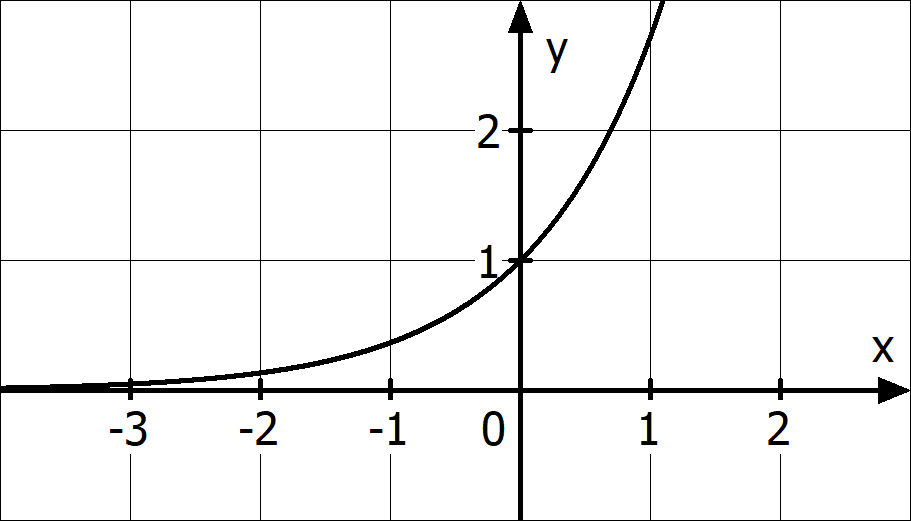
\includegraphics[width=.95\linewidth]{\eFkt/pics/ln.png}
\end{minipage}\vspace{0.2cm}
\begin{itemize}
	\item \(y\) ist größer 1 bzw. \(y>1\):\\
	\textcolor{loes}{Da \(e^x\) jeden \(y\)-Wert größer als 1 genau einmal annimmt und die passenden \(x\)-Werte alle positiv sind, darf man Zahlen größer 1 in den \(\ln\) einsetzen und das Ergebnis ist positiv:\\
		\(\ln(y)>0\) für \(y>1\)\\
		Bsp.: \(\ln(2)=0,693147\dots\)}
	\item \(y=1\):\\
	\textcolor{loes}{Der einzige Wert, den man auswendig können muss. Da \(e^0=1\) ist, gilt umgekehrt \(\ln(1)=0\)}\vspace{0.5cm}
	\item \(y\) liegt zwischen 0 und 1 bzw. \(0<y<1\):\\
	\textcolor{loes}{Da \(e^x\) jeden \(y\)-Wert zwischen 0 und 1 genau einmal annimmt und die passenden \(x\)-Werte alle negativ sind, darf man Zahlen zwischen 0 und 1 in den \(\ln\) einsetzen und das Ergebnis ist negativ:\\
		\(\ln(y)<0\) für \(0<y<1\)\\
		Bsp.: \(\ln(0,25)=-1,38629\dots\)}
	\item \(y\) ist kleiner gleich 0 bzw. \(y\leq0\):\\
	\textcolor{loes}{Da \(e^x\) niemals Null wird und auch keine negativen Funktionswerte annimmt, darf man weder Null noch eine negative Zahl in den \(\ln\) einsetzen:\\
		\(\ln(y)\) \Lightning \normalsize für \(y\leq0\)}
\end{itemize}
\newpage
%%%%%%%%%%%%%%%%%%%%%%%%%%%%%%%%%%
Es gibt zwar Rechengesetze für Logarithmen, wir werden diese aber nicht betrachten.\\
Zum Vergleichen von Lösungen kann aber folgendes Gesetz nützlich sein:
\begin{tcolorbox}\centering
	\(\textcolor{loestc}{\ln\left(\dfrac{a}{b}\right)=-\ln\left(\dfrac{b}{a}\right)}\)
\end{tcolorbox}
Mit Hilfe des natürlichen Logarithmus lassen sich Gleichungen mit Exponentialfunktionen mit Hilfe der gleichen Lösungsmethoden lösen, die wir auch bei ganzrationalen Funktionen bereits angewandt haben:
\begin{enumerate}[label=\arabic*)]
	\item Auflösen und \(\ln\) anwenden\\
	Dieses Verfahren kann nur dann angewendet werden, wenn die Gleichung auf folgende Form gebracht werden kann: \(ae^{kx}+b=0\)\\
	Wir lösen nach \(e^{kx}\) auf, d.h. \(e^{kx}\) steht alleine auf einer Seite. Dann wenden wir den \(\ln\) auf beiden Seiten an.\\
	Beispiel: Löse die Gleichung \(2e^{3x}-4=0\).
	\textcolor{loes}{\begin{align*}
			2e^{3x}-4&=0\ \vert\ +4\\
			2e^{3x}&=4\ \vert\ :2\\
			e^{3x}&=2\ \vert\ \ln\\
			3x&=\ln\left(2\right)\ \vert\ :3\\
			x&=\frac{1}{3}\ln\left(2\right)
	\end{align*}}
	\item Ausklammern und SvN\\
	Dieses Verfahren wenden wir dann an, wenn jeder Summand über ein \(e^{k_ix}\) verfügt. (Die \(k_i\) sind dabei paarweise verschieden.) Wir klammern ein \(e^{k_ix}\) vor (welches ist egal) und wenden dann den Satz vom Nullprodukt an.\\
	Beispiel: Löse die Gleichung \(2e^{3x}-4e^{7x}=0\).\\
	\begin{minipage}{\textwidth}\vspace{.15cm}
		\begin{minipage}[t]{0.49\textwidth}
			1. Möglichkeit
			\textcolor{loes}{\begin{align*}
					2e^{3x}-4e^{7x}&=0\\
					e^{3x}\left(2-4e^{4x}\right) &=0\\
					\text{SvN: Entweder }e^{3x}&=0 \text{\Lightning}\\
					\text{oder }2-4e^{4x}&=0\ \vert\ +4e^{4x}\\
					4e^{4x}&=2\ \vert\ :4\\
					e^{4x}&=\frac{1}{2}\ \vert\ \ln\\
					4x&=\ln\left(\tfrac{1}{2}\right)\ \vert\ :4\\
					x&=\frac{1}{4}\ln\left(\tfrac{1}{2}\right)
			\end{align*}}
		\end{minipage}
		\begin{minipage}[t]{0.49\textwidth}
			2. Möglichkeit
			\textcolor{loes}{\begin{align*}
					2e^{3x}-4e^{7x}&=0\\
					e^{7x}\left(2e^{-4x}-4\right) &=0\\
					\text{SvN: Entweder }e^{7x}&=0 \text{\Lightning}\\
					\text{oder }2e^{-4x}-4&=0\ \vert\ +4\\
					2e^{-4x}&=4\ \vert\ :2\\
					e^{-4x}&=2\ \vert\ \ln\\
					-4x&=\ln\left(2\right)\ \vert\ :(-4)\\
					x&=-\frac{1}{4}\ln\left(2\right)
			\end{align*}}
		\end{minipage}
	\end{minipage}
\end{enumerate}\newpage
\begin{enumerate}[label=\arabic*)]
	\setcounter{enumi}{2}
	\item Substitution\\
	Dieses Verfahren setzen wir dann ein, wenn die Gleichung auf folgende Form gebracht werden kann: \(ae^{2kx}+be^{kx}+c=0\)\\
	Wir substituieren \(z=e^{kx}\) und damit \(z^2=e^{2kx}\). Die entstehende quadratische Gleichung lösen wir mit Hilfe der Mitternachtsformel und erhalten dann die Lösungen für \(x\) nach einer Rücksubstitution.\\
	Beispiel: Löse die Gleichung \(0,5e^{6x}+e^{3x}-4=0\).
	\textcolor{loes}{\begin{align*}
			0,5e^{6x}+e^{3x}-4&=0\ \vert\ \text{Sub.: }z=e^{3x}\\
			0,5z^2+z-4&=0\\
			z_{1/2}&=\frac{-1\pm\sqrt{1^2-4\cdot 0,5\cdot \left(-4\right)}}{2\cdot 0,5}\\
			z_1&=-4\quad z_2=2\ \vert\ \text{Rücksub.}\\
			e^{3x}&=-4\text{ \Lightning\normalsize oder}\\
			e^{3x}&=2\ \vert\ \ln\\
			3x&=\ln\left(2\right)\ \vert\ :3\\
			x&=\frac{1}{3}\ln\left(2\right)
	\end{align*}}
\end{enumerate}
\newpage
%%%%%%%%%%%%%%%%%%%%%%%%%%%%%%%%%%%%%%%%%%%%%%%%%%%%%%%%%%%%%%%%%%%%%%%%%%%%%%%%%%%%%%%%%%%%%%%%%%%%%%
\begin{Exercise}[title={Löse folgende Gleichungen}, label=eFktGlA1]\\
	\begin{minipage}{\textwidth}
		\begin{minipage}{0.49\textwidth}
			\begin{enumerate}[label=\alph*)]
				\item \(3e^x-9=0\)
				\item \(4e^{3x}-12=0\)
				\item \(5e^{4x}-2e^{x}=0\)
				\item \(0,5e^{-2x}+e^{-x}-12=0\)
				\item \(3e^{-8x}+6=0\)
				\item \(-\frac{3}{4}e^{-\tfrac{2}{3}x}+12=0\)
				\item \(e^{8x}-5e^{4x}+10=0\)
				\item \(-e^{x}+0,4=0\)
				\item \(-10e^{10x}-13e^{5x}-4=0\)
				\item \(7-e^{-2x}=0\)
				\item \(7e^{-4x}-e^{-2x}=0\)
				\item \(-2e^{-6x}+\frac{13}{2}e^{-3x}-\frac{3}{2}=0\)
				\item \(5e^{4x}-10e^{-x}=0\)
			\end{enumerate}
		\end{minipage}
		\begin{minipage}{0.49\textwidth}
			\begin{enumerate}[label=\alph*)]
				\setcounter{enumi}{13}
				\item \(0,4e^{4x}+1,8e^{2x}=0\)
				\item \(-3e^{4x}+8e^{-2x}=0\)
				\item \(e^{2x}+2e^{x}-3=0\)
				\item \(3e^{3x}+\frac{1}{2}e^{1,5x}-\frac{1}{2}=0\)
				\item \(e^{5x}-4e^{\tfrac{5}{2}x}-12=0\)
				\item \(-\frac{2}{3}e^{4x}-e^{x}=0\)
				\item \(-0,2e^{0,3x}-1,4=0\)
				\item \(2e^{-2x}+e^{-x}-6=0\)
				\item \(5e^{-6x}=4\)
				\item \(0,1e^{4x}-e^{x}=0\)
				\item \(-\frac{1}{9}e^{-0,5x}+\frac{2}{3}e^{-0,25x}=-3\)
				\item \(0,5e^{4x}=e^{x}\)
				\item \(-3e^{x}+2=-e^{2x}\)
			\end{enumerate}
		\end{minipage}
	\end{minipage}
\end{Exercise}
\newpage
%%%%%%%%%%%%%%%%%%%%%%%%%%%%%%%%%%%%%%%%%
\begin{Answer}[ref=eFktGlA1]\\
	\begin{minipage}{\textwidth}
		\begin{minipage}{0.49\textwidth}
			\begin{enumerate}[label=\alph*)]
				\item \(x=\ln\left(3\right)\)
				\item \(x=\frac{1}{3}\ln\left(3\right)\)
				\item \(x=\frac{1}{3}\ln\left(\frac{2}{5}\right)=-\frac{1}{3}\ln\left(\frac{5}{2}\right)\)
				\item \(x=-\ln\left(4\right)\)
				\item keine Lösung
				\item \(x=-\frac{3}{2}\ln\left(16\right)\)
				\item \(x_1=\frac{1}{4}\ln\left(2\right),\ x_2=\frac{1}{4}\ln\left(3\right)\)
				\item \(x=\ln\left(0,4\right)\)
				\item keine Lösung
				\item \(x=-\frac{1}{2}\ln\left(7\right)\)
				\item \(x=-\frac{1}{2}\ln\left(\frac{1}{7}\right)=\frac{1}{2}\ln\left(7\right)\)
				\item \(x_1=-\frac{1}{3}\ln\left(3\right),\ x_2=-\frac{1}{3}\ln\left(\frac{1}{4}\right)\)
				\item \(x=\frac{1}{5}\ln\left(2\right)=-\frac{1}{5}\ln\left(\frac{2}{1}2\right)\)
			\end{enumerate}
		\end{minipage}
		\begin{minipage}{0.49\textwidth}
			\begin{enumerate}[label=\alph*)]
				\setcounter{enumi}{13}
				\item \(x=0,5\ln\left(4,5\right)=-0,5\ln\left(\frac{2}{9}\right)\)
				\item \(x=\frac{1}{6}\ln\left(\frac{8}{3}\right)=-\frac{1}{6}\ln\left(\frac{3}{8}\right)\)
				\item \(x=0\)
				\item \(x=\frac{2}{3}\ln\left(\frac{1}{3}\right)\)
				\item \(x=\frac{2}{5}\ln\left(6\right)\)
				\item keine Lösung
				\item keine Lösung
				\item \(x=-\ln\left(\frac{3}{2}\right)\)
				\item \(x=-\frac{1}{6}\ln\left(\frac{4}{5}\right)\)
				\item \(x=\frac{1}{3}\ln\left(10\right)=-\frac{1}{3}\ln\left(\frac{1}{10}\right)\)
				\item \(x=-4\ln\left(9\right)\)
				\item \(x=\frac{1}{3}\ln\left(2\right)=-\frac{1}{3}\ln\left(0,5\right)\)
				\item \(x_1=\ln\left(2\right),\ x_2=0\)
			\end{enumerate}
		\end{minipage}
	\end{minipage}
\end{Answer}